%% LyX 2.2.3 created this file.  For more info, see http://www.lyx.org/.
%% Do not edit unless you really know what you are doing.

\documentclass[10pt,twocolumn,american]{article}
\usepackage[sc]{mathpazo}
\usepackage[scaled=0.9]{helvet}
\renewcommand{\ttdefault}{lmtt}
\usepackage[T1]{fontenc}
\usepackage[latin9]{inputenc}
\usepackage[a4paper]{geometry}
\geometry{verbose,lmargin=1.7cm,rmargin=1.7cm}
\usepackage{fancyhdr}
\pagestyle{fancy}
\setcounter{secnumdepth}{0}
\setcounter{tocdepth}{3}
\setlength{\parskip}{\smallskipamount}
\setlength{\parindent}{0pt}
\usepackage{babel}
\usepackage{float}
\usepackage{enumitem}
\usepackage{graphicx}
\usepackage{titlesec}
\usepackage{todonotes}
\usepackage[unicode=true,
 bookmarks=true,bookmarksnumbered=false,bookmarksopen=false,
 breaklinks=false,pdfborder={0 0 0},backref=false,colorlinks=false]
 {hyperref}
\usepackage{amsmath}
\usepackage{nicefrac}
\usepackage{ulem}
\makeatletter

% User specified LaTeX commands.
% Customization file for the titlepage and document
%************************************************************
% Required stuff
%************************************************************
\usepackage{graphicx}
\usepackage{euler}
\usepackage[detect-all]{siunitx}
\usepackage{sectsty}
\usepackage[font={footnotesize }]{caption}
\usepackage{multicol}
\usepackage{prettyref}

\allsectionsfont{\rmfamily}

% Page customization
\usepackage{fancyhdr}
\pagestyle{fancy}

% Color
\usepackage{color}
\definecolor{light-gray}{gray}{0.85}
\definecolor{dark-gray}{gray}{0.75}

\fancyhead{}  % clear all header fields
\fancyhead[LO,RE]{\rule[-2ex]{0pt}{2ex}\fontsize{9}{11} \selectfont \myPhase : \myTitle}
\fancyhead[CO,CE]{\fontsize{9}{11} \selectfont \myIPT}
\fancyfoot{}  % clear all footer fields
\fancyfoot[LO,LE]{\fontsize{8}{11} \selectfont {\sscap{Website}} : \url{https://github.com/fcuzzocrea/MSAS2017}}
\fancyfoot[RO,LE]{\fontsize{5}{11} \selectfont 
\includegraphics[height=0.18cm]{gfx/CC}  This work is licensed under a Creative Commons Attribution-ShareAlike 4.0 International License.}
\fancyheadoffset[LE,RO]{0.2pt}
\renewcommand{\headrulewidth}{0.2pt}
\renewcommand{\footrulewidth}{0.2pt}
\renewcommand{\headrule}{\hbox to\headwidth{%
   \leaders\hrule height \headrulewidth\hfill}}
\renewcommand{\footrule}{\hbox to\headwidth{%
    \leaders\hrule height \headrulewidth\hfill}}
\hypersetup{colorlinks=true, linkcolor=blue ,linktoc=page,citecolor=black}

%************************************************************
% Redefining numbering for sections
%************************************************************
%\renewcommand*\thesection{\arabic{section}}

%************************************************************
% Cross reference set-up
%************************************************************
\newrefformat{tab}{Table\,\ref{#1}}
\newrefformat{fig}{Figure\,\ref{#1}}
\newrefformat{eq}{Eq.\,\textup{(\ref{#1})}}
\newrefformat{sec}{Sec.\,\ref{#1}}
\newrefformat{sub}{Sec.\,\ref{#1}}

%************************************************************
% Fancy stuff
%************************************************************
\newcommand{\titlecap}[1]{\Huge{\textrm{#1}}}
\newcommand{\subtitlecap}[1]{\Large{\textsc{#1}}}
\newcommand{\sscap}[1]{\textbf{#1}}
\newcommand{\strong}[1]{\textbf{#1}}
\setlength{\headheight}{60pt} %%or

%************************************************************
% Helpful stuff to modify here, not in the LyX Document
%************************************************************
\newcommand{\myDate}{\today}
\newcommand{\myGroup}{}
\newcommand{\myUrl}{\url{https://github.com/fcuzzocrea/MSAS2017}}
\newcommand{\myUni}{}

\newcommand{\myPhase}{Modeling and Simulation of Aerospace Systems}
\newcommand{\myProject}{}
\newcommand{\myIPT}{}
\newcommand{\myTitle}{LISA Pathfinder Final Report}
\newcommand{\myAuthorf}{Alfonso Collogrosso}
\newcommand{\myAuthors}{Francescodario Cuzzocrea}
\newcommand{\myAuthort}{Andrea Mastrantuono}
\newcommand{\myEmail}{}

\newcommand{\mail}[1]{\href{mailto:#1}{\texttt{#1}}}

\setlength{\textfloatsep}{\baselineskip}

\makeatother

\begin{document}

\title{ \titlecap{\Large \myPhase} \rule{\linewidth}{0.01mm}  {\myTitle}}
\date{\today}
\author{\textbf{Authors} : {\myAuthorf, \myAuthors, \myAuthort}}

% Put the abstract fullpage
\twocolumn[
\begin{@twocolumnfalse}
	\maketitle
	\rule{\linewidth}{0.5mm}
		\begin{abstract}
			The LISA scientific space mission will detect gravitational waves by measuring the relative displacement of a pairs of free floating test masses set into geodesic motion on-board of three spacecraft. Inside each satellite, the injection of the test masses from the caged configuration into the geodesic trajectory will be performed by the Grabbing Positioning and Relased Mechanism (GPRM). To provide a successful injection, the test masses must be relased with a minimal residual velocity against the adhesion with the holding device.
In the following document we will proceed trough the derivation and the integration of the system of linear ODEs that describes the forementioned grabbing positioning and relase mechanism.

		\end{abstract}
	\rule{\linewidth}{0.5mm}
\end{@twocolumnfalse}
]

\pagenumbering{arabic}

\setcounter{secnumdepth}{3}

\section{Introduction}
	The LISA (Laser Interferometer Space Antenna) Pathfinder mission is a scientific mission aimed at revealing gravitational waves by means of the formation distortion of 3 \textit{Test Masses} (TMs), each one in a different spacecraft, put in a free-falling (geodesic) trajectory.\\
	Due to weak gravitational waves interaction, any force different from gravitational ones acting on TMs must be negligible, and the TM release must meet the requirements listed in tab.1:
	
	\begin{table}[H]
	\renewcommand{\arraystretch}{1.1}
		\begin{centering}
			\begin{tabular}{l|l} \hline
				parameter & tolerance \\ \hline
				offset along x, y and z & $\pm 200 \mu m$\\
				linear velocity along x, y and z & $\pm 5 \mu m/s$\\
				angle around x, y and z & $\pm 2 mrad$\\
				angular velocity around x, y, z& $\pm 100 \mu rad/s$\\ 
			\end{tabular}
		\end{centering}
		\caption{requirements for TM release}
	\end{table}

\section{Modeling}
	\subsection{The real system}	
	The LISA Pathfinder Grabbing Position and Relase Mechanism (GPRM) is the system aimed to lock and relase the TM into the spacecraft. 
	In fact, the forementioned TM has to be relased with a nearly zero velocity with respect to the transport spacecraft in order to be correctly injected into a geodesic trajectory. \\
	This task can be relatively complex, if we think of the possible interactions developing with the support, and because of the electrostatic aspects that may generate disturbing forces. \\
	Also, least but not last, the quality of the surface of the test mass and of the grabbing finger should be taken into account. \\ 
	The GPRM mechanism is sketched in Fig 1.
		
	\begin{figure}[H]
		\begin{centering}
			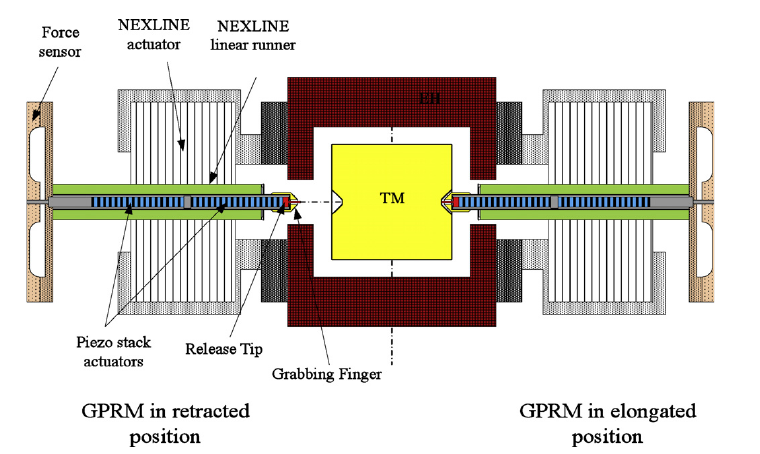
\includegraphics[scale=0.4]{gfx/GPRM}
		\end{centering}
		\caption{GPRM Mechanism}
	\end{figure}
	
	Its main parts are:
	\begin{itemize}
		\item \textit{Grabbing Finger}: holds the TM and positions it prior relase;
		\item \textit{Finger Tip}: last contact part that pons the TM in position before fast retraction for relase;
		\item \textit{Low Voltage Piezo Actuator}: used for the positioning and fast Finger Tip relase;
		\item \textit{NEXLINE actuator}: used for Grabbing Finger movement;
		\item \textit{Displacemente Sensor}: to measure the axial force acting between the mechanism contacting interface;
	\end{itemize}

	\subsubsection*{Main Task}
	The model of the injection procedure consists of three parts.\\
	The GPRM, the adhesion phoenomenon and the TM motion equations.
	Two opposite GPRMs are operated simultaneously in order to hold the
	TM with the Grabbing Fingers in the center of the Electrode Housing
	(EH). From this configuration, the procedure can be considered to be symmetrical, as the two mechanism are commanded in the same way:	
	\begin{itemize}
		\item \textbf{Pre-launch and launch phase}
		\begin{enumerate}
			\item The TM is held by the Caging Mechanism (CM) at the eight corners;
		\end{enumerate}
		\item \textbf{TM Release from CM}
		\begin{enumerate}
			\item The Grabbing Finger is in contact with the TM and the tip is fully retracted;
		\end{enumerate}
	\end{itemize}	
	The contact between the GF and the TM has to perform the following
	functions :	
	\begin{description}
		\item [{-}] Fix the TM during the release of the CM;
		\item [{-}] Center the TM in the EH;
		\item [{-}] Orient the TM with respect to the EH;
	\end{description}	
	This contact however not suitable for an undisturbated release for geodesic injection.\\ 
	The release tip must thus take over the TM pinning before
	release. 	
	\begin{itemize}
		\item \textbf{Pass Over}
		\begin{enumerate}
			\item The RT moves forward until a contact force is recorded 
			\item The GF is	retracted a small amount to compensate for the movement of the RT;
			\item The force is then reduced to the lowest acceptable level that still controls the position of the TM;
			\item TM release is performed by means of a fast contraction of the linear piezo actuator, which also commands the retraction of the tips;
			\item The TM is capture by the drag-free attitude and control system and take finally to the 					nominal center of its housing;
		\end{enumerate}
	\end{itemize}	
	We must pay attention to the fact that in presence of adhesion the
	fast retraction may cause a momentum transfer from the RTs to the TM. 

\subsection{The Physical System}
    The GPRM can be physically modeled as the lumped-element diagram reported in Figure 2 :  
    
    	\begin{figure}[H]
		\begin{centering}
			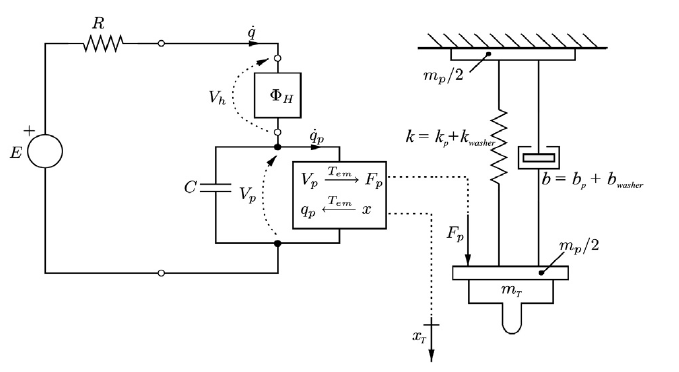
\includegraphics[scale=0.4]{gfx/phys_model}
		\end{centering}
		\caption{GPRM Physical Model}
	\end{figure}
	
	The diagram comprises the release tip mass and washer springs mounted at the extremity of the Grabbing Finger (GF) unit, and the piezo-stack actuator connected to a voltage generator through a discharge resistor R.
	
\subsection{The Mathematical Model}
\subsubsection*{Release tip model}
    A mathematical model for the lumped-element freshly shown can be easily derived by resorting to elementary physical laws, such as the Kirchoff laws and Newton's laws, once the constitutive equations of the piezo-stack actuator are known.
    The most conventional model of a piezo-stack actuator is the one which relies on the linear constitutive equations of piezoelectric materials. \todo[inline]{inserire citazione paper} 
    Such model however is not useful for describing the dynamics of piezo-actuated positioning mechanisms because it neglects the intrinsic dynamics of the actuator. 
    A lumped parameter linear model for the piezo actuator can be obtained by manipulating the equations provided in \todo[inline]{inserire citazione paper isteresi} and by neglecting the hysteresis \todo[inline]{inserire citazione paper bortoluzzi 1} .\\
    Using the Newton and Kirchoff's laws, together with the constitutive equations of the piezoelectric transducer, and by neglecting the degree of freedom describing the suspended mass of the piezo stack\todo[inline]{inserire citazione paper bortoluzzi 2} we can obtain the equations governing the simplified model of Fig. 2 :
    \begin{equation}
        RC_{a}\dot{q}(t)+q(t)-T_{em}x_{T}(t)=C_{a}E(t)
    \end{equation}
    
    \begin{equation}
        m\ddot{x}_{T}(t)+ b\dot{x}_{T}(t) + \left(k+\frac{T_{em}^{2}}{C_{a}}\right) x_{T}(t) - \frac{T_{em}}{C_{a}}q(t) = 0
    \end{equation}
    where :
	\begin{itemize}
		\item $E(t)$ is the input voltage
		\item $q(t)$ is the charge accumulated on the piezo
		\item $x_{T}(t)$ is the RT position
		\item $C_{a}$ is the capacitance of the piezo stack
		\item $T_{em}$ is the piezo effect
		\item $m$ is the mass of the RT plus half of the mass of the piezo-stack
		\item $b$ is the damping coefficient
		\item $k$ is the stiffness coefficient
	\end{itemize}
    If the voltage $E$ and the test mass displacement $x_{T}$ are taken as the input and output variables of the system, then we can write the transfer function describing the dynamics of the GPRM as :
    \begin{equation}
        G(s) = \frac{X(s)}{E(s)} = \frac{b_{2}s^{2}+b_{1}s+b_{0}}{a_{5}s^{5}+a_{4}s^{4}+a_{3}s^{3}+a_{2}s^{2}+a_{1}s+a_{0}}
    \end{equation} 
    The system may be written in state space as\\
    \begin{frame}
        \footnotesize
        \setlength{\arraycolsep}{2.5pt}
        \medmuskip = 1mu
        \thickmuskip = 1mu
        \small\[\scriptstyle 
        \left(\begin{array}{@{}c@{}}
        \dot{q}_{T}(t)\\
            \dot{x}_{T}(t)\\
            \ddot{x}_{T}(t)
            \end{array}\right)=\left[\begin{array}{@{}ccc@{}}
            -\frac{1}{C_{a}R} & \frac{T_{em}}{C_{a}R} & 0\\
            0 & 0 & 1\\
            \frac{T_{em}}{C_{a}m} & -\frac{k}{m}-\frac{T_{em}^{2}}{C_{a}m} & -\frac{b}{m}
            \end{array}\right]\left(\begin{array}{c}
            q(t)\\
            x_{T}(t)\\
            \dot{x}_{T}(t)
            \end{array}\right)+\left(\begin{array}{@{}c@{}}
            \frac{1}{R}\\
            0\\
            0
        \end{array}\right)E(t)
              \]
    \end{frame}

    \begin{frame}
        \footnotesize
        \setlength{\arraycolsep}{2.5pt}
        \medmuskip = 1mu
        \thickmuskip = 1mu
        \small\[\scriptstyle 
            {y}(t) = 
            \left[\begin{array}{@{}ccc@{}}
            0 & 1 & 0\\
            \end{array}\right]\left(\begin{array}{@{}c@{}}
            q(t)\\
            x_{T}(t)\\
            \dot{x}_{T}(t)
            \end{array}\right)
                \]
    \end{frame}
  where the elements $A_{1,1}$, $A_{1,2}$, $A_{3,1}$, $A_{3,2}$, $A_{3,3}$, $B_{1}$ are unknown and will be estimated in identification (Sec 3.1).
  \subsubsection*{Test mass model}
 TM is easily modeled as a rigid body in free motion, Newton's equations describe linear displacement dynamics
 \begin{equation*}
 M\uline{\ddot{x}}_{TM} = \uline{F}
 \end{equation*} 
 while Euler's equations
 \begin{equation*}
 \uuline{J}\uline{\dot{\omega}}+\uuline{J}\uline{\omega}\times\uline{\omega}=\uline{M}
 \end{equation*}
 can be simplified in this case since inertia moment I is the same for each of the 3 principal axes ($J_{i,j} =I \delta_{i,j}$) and describe angular dynamics
 \begin{equation*}
 I\uline{\dot{\omega}}=\uline{M}
 \end{equation*}
 To complete the model, a set of kinematic equations for angular motion shall be considered
 \begin{equation*}
 \uuline{\dot{A}}+\uuline{\big[\omega^{\wedge}\big]}\uuline{A} =0
 \end{equation*}
 This last equation can be substituted by different models i.e. Euler Angles kinematic equations that can be more suitable. A simplified model have been derived considering system simmetry. Force components on y and z axes arise due to TM rotation. Angular velocity is expected to be of the order of few $\mu rad/s$, the contact between TM and RTs lasts much less than $1 ms$, as a result rotation angle is a fraction of $nrad$ and his effects on contact force are neglected. Morover, rotation arises for a modeled misalignment on y-axis only the rotational dynamics and kinematics as well as the linear ones occur on one axis only. The system is therefore widely symplified:
 \begin{align}
 &M\ddot{x}_TM=F\\ 	
 &I\dot{\omega}=M\\ 
 &\dot{\theta}=\omega
 \end{align}
  \subsubsection*{Adhesion force model}
  \begin{table*}
  \setlength{\tabcolsep}{0.35 cm}
  \renewcommand{\arraystretch}{1.2}
  \begin{tabular}{c| c c|c c|c c }
  \textbf{Coefficient} & \multicolumn{2}{c|}{\textbf{set 1}}&\multicolumn{2}{c|}{\textbf{set 2}}& \multicolumn{2}{c}{\textbf{set 3}}\\
  &mean value & std.dev. & mean value & std.dev. &mean value & std.dev. \\ \hline
  $X_1$& $0.503$&$2.59 \times 10^{-2}$ & $ 0.357$ & $ 7.30 \times 10^{-2}$ &$0.457$ & $3.58 \times 10^{-2}$\\
  $X_2$ & $2.89$ & $2.75 \times 10^{-1}$ & $1.32$ & $1.59\times 10^{-1}$ & $1.73$ & $1.22\times 10^{-1}$\\
  $X_3$ & $2.36$ & $4.76\times 10^{-2}$ & $2.07$ & $2.14 \times 10^{-1}$ & $1.27$ & $2.98 \times 10^{-1}$\\
  \end{tabular}
  \caption{adhesion force fitting results}
  \end{table*}
  The following description of the adhesion force competes the model. A dynamic model for tip actuation and TM motion has been derived and it includes a parametric representation of force acting on tip and which is an input of the system. The description of adhesion force starts with experimental data shown in Fig. 3, that presents several experimental measurments for 3 different sets. 
\begin{figure}[t]
		\begin{centering}
			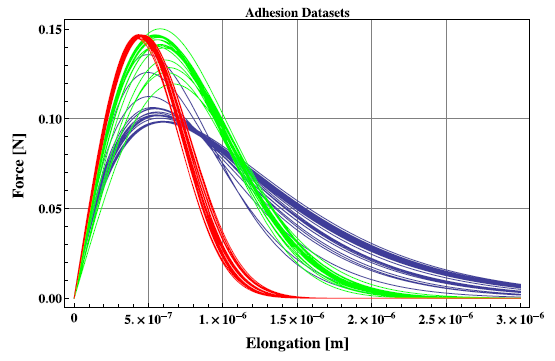
\includegraphics[scale=0.6]{gfx/adh_data}
		\end{centering}
		\caption{Adhesion force experimental data (from Bortoluzzi et al. 2012)}
	\end{figure}
Following the procedure adopted by Bortoluzzi  \todo[inline]{inserire citazione paper bortoluzzi 2}, once experimental data are sampled from Fig.3, they are fitted into exponential model:\\
\begin{equation*}
  F_{ad}(\Delta l)=X_1\Delta l e^{X_2\Delta l^{X_3}} \\
  \end{equation*}
The MATLAB \textbf{lsqcurvefitting} routine is then used to perform a least square minimization fitting of the experimental data. Resulting $X_1,X_2,X_3$ coefficients and their standard deviations are listed in table 2.
\begin{figure}[t]
		\begin{centering}
			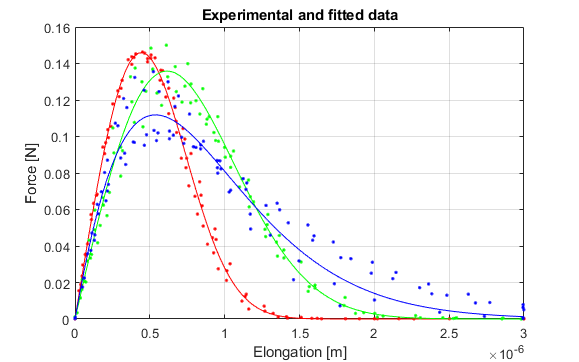
\includegraphics[scale=0.6]{gfx/adh_all}
			
		\end{centering}
		\caption{Adhesion force sampled data and fittings}
\end{figure}
\subsubsection*{Contact force model and preload}
During \textit{pass-over} operation (Sec. 2.1), just before TM release, RT reduces the force on TM to the lowest acceptable level that still controls the TM, generating a preload on the RT. This value is of the order of 0.1N \todo[inline]{bortoluzzi 1 2}, in this report is considered 0.3N. The presence of the preload alters the initial elongation of RT which is easily computed solving the steady state system for release tip:
\begin{equation*}
\uuline{A}\uline{x} + \uuline{B}
\begin{pmatrix}
E_0\\F_0
\end{pmatrix}
 = 0\\
\end{equation*}
being $E_0 = 120 V$ and $F_0 = 0.3 N$ initial steady state input vector components.\\
Another issue is to model the force between TM and RT. This force in an ideal point of view is a dirac delta of the elongation (reaction force different from 0 for 0 elongation only), but for numerical reasons it must be described as a continous function. The following description is then adopted, depicted in figure \todo[inline]{figure number}, considering $\Delta l$ in $\mu m$\\
\begin{align*}
&F = 0.3N & &\text{if} & &\Delta l <0\\
&F =( -3\times 10^2 + 0.3) N & &\text{if} & 0< &\Delta l<10^{-3}\\
&F = 0N & &\text{if} & &\Delta l>10^{-3}
\end{align*}
\begin{figure}
		\begin{centering}
			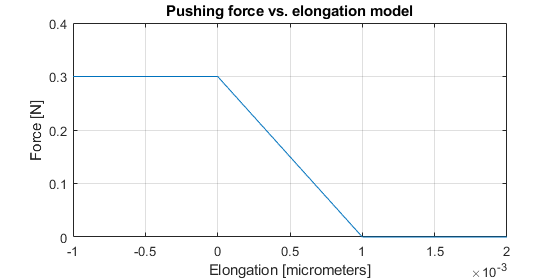
\includegraphics[scale=0.6]{gfx/Push_mdl}
			
		\end{centering}
		\caption{Model of the pushing force as function of the elongation}
\end{figure}
Provided that central linear part passes to point (0,0.3), so that the description exploits the fact that largest RT pushing force on TM is $0.3N$ (unloading spring like behaviour), only one parameter is arbitrary: the elongation at which F goes to zero (the treshold at which pushing force starts to act), here chosen as $\Delta l = 10^{-3} \mu m$. The choice of this parameter is driven by the following considerations:
\begin{enumerate}
\item{push force must not occur when adhesion force is acting, so max. $10^{-2}$ considering that adhesion force has a maximum around $10^{-1} \mu m$}
\item{In \todo[inline]{bortoluzzi 2} there is a depiction of RT surface roughtness}
\item{Simulation results variation is small if the parameter is chosen in a certain domain, which is approximately $[10^{-4} : 10^{-2}] \mu m$}
\end{enumerate}
\section{Simulation}
\begin{table*}[t]
\setlength{\tabcolsep}{0.5 cm}
\renewcommand{\arraystretch}{1.2}
\begin{tabular}{|c |c c c c c|}\hline
parameter & guess value & lower bound & upper bound & identified value & units \\ \hline
$C_a$ & $4.8\times 10^{-7}$ & 0 & $10^{-6}$ & $3.936 \times 10^{-7}$ & F \\
$T_{em}$ & $1.5$ & 0 & - & $1.51$ & $\sqrt{\nicefrac{FN}{m}}$ \\
R & 400 & 100 & 800 &417 & $\Omega$\\
m & $10^{-3}$ & $10^{-4}$ &0.014 & $10^{-4} $ & kg\\
b & 150 & 100 & - & 100 & $\nicefrac{Ns}{m}$ \\
k & $1.5 \times 10^7$ & 0 & - & $1.5 \times 10^7$ & $\nicefrac{m}{s}$\\
$V_0$ & 0 & -0.05 & 0.05 & $3 \times 10^{-3}$ & $\nicefrac{m}{s}$ \\ \hline
\end{tabular}
\caption{Identification inputs and results}
\end{table*}
\subsection{Identification}
Identification makes use of experimental data to estimate unknown parameters of the model. Experimental data are extrapolated from \todo[inline]{inserire citazione paper bortoluzzi 2} and are resampled with a 1MHz frequency to be consistent with the cited paper data. 
The parameters to be identified are the six physical constants that appear nonlinearly in RT linear system, the $V_0$ initial velocity of the RT parametrized as: \\
\\
\begin{centering}
$
\begin{pmatrix}
q(0) \\
x_T(0) \\
\dot{x}_T(0)
\end{pmatrix}
=
\begin{pmatrix}
0 \\
0 \\
V_0
\end{pmatrix}
$
\end{centering}
\\
\\
Therefore, the vector of parameters to be estimeted is defined as:\\
\\
\begin{centering}
$\textbf{p} = 
\begin{bmatrix}
C_a \\
T_{em} \\
R \\
m \\
b \\
k \\
V_0
\end{bmatrix}
$
\end{centering}
\\
\\
Identification consists in minimaze the variance of the residual between measured and modeled responce:\\
\\
$ \textbf{p}=argmin(\psi_N(\textbf{p}))$\\
\\
with penalty function $\psi_N$ defined as:\\
\\
$\psi_N(\textbf{p})=\frac{1}{N}\sum\limits_{i=1}^N(y_N(t_i)-y(t_i|\textbf{p}))^2$\\
where $y_N$ is the experimental responce and $y(t_i|\textbf{p})$ is the modeled responce with parameter set \textbf{p}.\\
Identification is performed with MATLAB \textbf{pem} command using the Levenberg-Marquardt search method. Due to non linearity of the problem many local minima can be found and  in order to have the routine converging to a solution with physical meaning appropriate initial guess for \textbf{p} must be set, as well as suitable constrains (i.e. a lower bound to avoid physical parameters converging to a negative value). \\
\begin{figure}
		\begin{centering}
			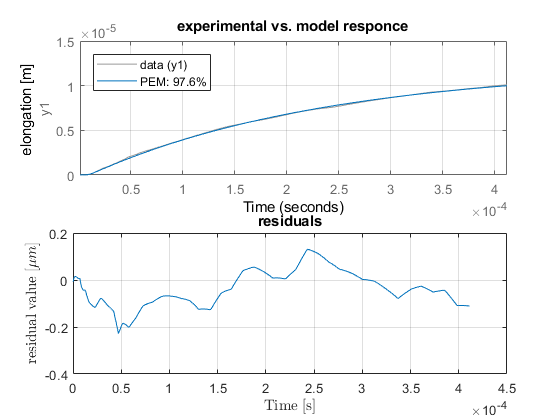
\includegraphics[scale=0.6]{gfx/Identification_results}
		\end{centering}
		\caption{Comparison between modeled and experimental responce}
\end{figure}
Estimated parameters are reported in Table 3. Figure 4 shows the comparison between experimental and identified model responce. Residuals are small, always <1\% of max. tip retraction, their RMS is $x_{T,rms}=84 nm$.\\

\subsection{Monte Carlo simulation}
In Sec. 3.1 nominal values of tip actuation mechanism parameters have been estimated. However some deviation of the actual mechanism from the nominal one may occur. In particular uncertainties arise from identification uncertainties and \textit{a priori} variance of parameters, uncertainty on contact force coefficients (which is a poorly repeatble phoenomenon), initial misalignment of RTs with respect to TM baricenter and asymmetry coming from a time lag on RT actuation. In order to generate an angular momentum on TM, an initial misalignment RTs is considered as a gaussian distribution with standard deviation $\sigma=100 \mu m$, which is $\nicefrac{1}{10}$ of RT emispheric contact surface diameter ($d = 1 mm$).
 The simulation is performed through a Monte-Carlo approach, repeating many times, 5000 times for each of the 3 adhesion force fittings, changing the model of the mechanism. The results of this procedure will be the \textit{Probability Density Function} of linear and angular velocities. 
\subsubsection*{Parameters uncertainty}
Two approaches are followed to include parameters uncertainty into the simulation.\\
The first one consists in letting each parameter assume in each simulation a random value with a suitable probability distribution. A covariance matrix is computed with the formula:\\
\begin{equation*}
\Sigma_p=\big(J^T\Sigma_x^{-1}J\big)^{-1}
\end{equation*}
where J is the jacobian. Being $x_i$ the retraction at i-th time step and $p_j$ the j-th parameter, J is defined as:\\
\begin{equation*}
J_{ij}=\frac{\partial x_i}{\partial p_j}\\
\end{equation*}
Jacobian is estimated by performing simulations of the nominal mechanism and of the mechanism with a parameter shifted from nominal one with an high order integrator (MATLAB routine \textit{ode113} was adopted for this purpose) and then comparing the responces. Being $res_i$ the residual at i-th time step, $\Sigma_x$ is built as:
\begin{equation*}
\Sigma_x = 
\begin{pmatrix}
res_1^2& 0 & \cdots & 0\\
0 & res_2^2 & \cdots & 0\\
\vdots & \vdots & \ddots & \vdots \\
0 & 0 & \cdots & res_N^2
\end{pmatrix}
\end{equation*}\\
A final form for covariance matrix accounts both for identification and \textit{a priori} uncertainties, here quantified as standard deviation $\sigma_0=0.3\times p$ for each parameter. Being $\Sigma_{p,0}^{-1}$ the a priori covariance matrix, covariance matrix is then defined as:
\begin{equation}
\Sigma_p=\big(\Sigma_{p,0}^{-1}+J^T\Sigma_x^{-1}J\big)^{-1}
\end{equation}
Eventually no correlation is assumed, so off-diagonal elements are ignored.\\
The main issue with this approach is the inversion on right hand side in equation \todo[inline]{put previous equation number}, which may yield inaccurate results. In this case, although high conditioning number, results appear consistent. The second approach consists in altering the tip retraction dynamics by a fotce F(t) applied on the tip which generates a displacement with same \textit{Power Spectral Density} (PSD) as the residual. The procedure is depicted in the main steps as follows:

\begin{align*}
r&es & &\text{residuals}\\ 
&\Downarrow \\
C_{res,res}&=res \ast res & &\text{auto correlation}\\ 
&\Downarrow \\ 
PSD_{2-sided}&=fft(C_{res,res}) & &\text{Fourier transform}\\
&\Downarrow \\
PSD\times n_w(j\omega)&=res_{rand} &&\text{white noise filtering}\\
&\Downarrow \\
F_{rand}(j\omega)&=\frac{res_{rand}}{H(j\omega)} &&\text{force in Fourier domain}\\
&\Downarrow\\
F_{rand}(t)&=ifft(F_{rand}(j\omega)) &&\text{force in time domain}
\end{align*}
Residual auto-correletion is transformed into Fourier domain to get the PSD, shown in \todo[inline]{inserire numero figura PSD}. Then a white noise, in frequency domain too, is filtered through the PSD. The filtered noise is a simulated random displacement, in order to use it in the simulation, it must pass through the \textit{Frequency Responce Function} (FRF), here called $H(j\omega)$, whose expression is stated below:
\begin{equation*}
H(j\omega)=\frac{X(j\omega)}{F(j\omega)}=\frac{b(j\omega)+1}{a_3(j\omega)^3+a_2(j\omega)^2++a_1(j\omega)+a_0}\\
\end{equation*}
where:
\begin{align*}
b& = R C_a\\
a_0&=k\\
a_1&=b+RT_{em}^2+RC_ak\\
a_2&=m+RbC_a\\
a_3&=RC_am
\end{align*}
The result is the random force to be applied on the tip in Fourier domain. \todo[inline]{inserire numero figura quantità in dominio di Fourier} shows FRF, displacement and force in frequency domain.Eventually the force is turned in time domain using inverse Fourier transform (\todo[inline]{inserire numero figura forza}).
\begin{figure}[H]
		\begin{centering}
			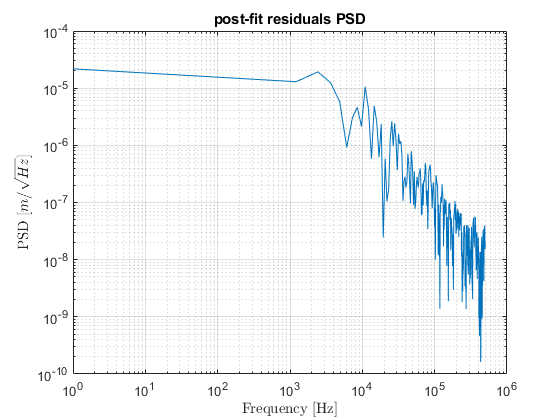
\includegraphics[scale=0.6]{gfx/PSD}
		\end{centering}
		\caption{residuals 1-sided PSD in logaritmic plot}
\end{figure}

This method has two main numerical criticalities:
\begin{enumerate}
\item The procedure described would be mathematically exact if signals to process where infinite in extension. The fact that the bandwidth is limited to [$-5\times10^5- 5\times10^5$]Hz (1MHz sampling frequency) is not critical because of the low-pass fiter like PSD behaviour is such that higher frequences would be filtered out anyway. On the other hand the residual is finite and this makes the auto-convolution inaccurate.
\item Displacement noise is divided by $H(j\omega)$, which is an FRF with a zero and may lead to numerical issues.
\end{enumerate}

\begin{figure}[H]
		\begin{centering}
			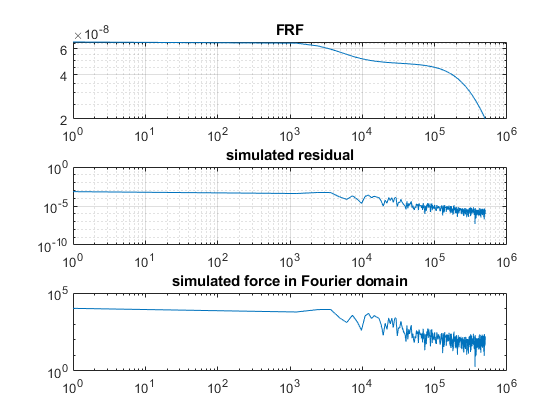
\includegraphics[scale=0.6]{gfx/F_domain}
		\end{centering}
		\caption{FRF and examples of residual and force in Fourier domain}
\end{figure}
\begin{figure}[H]
		\begin{centering}
			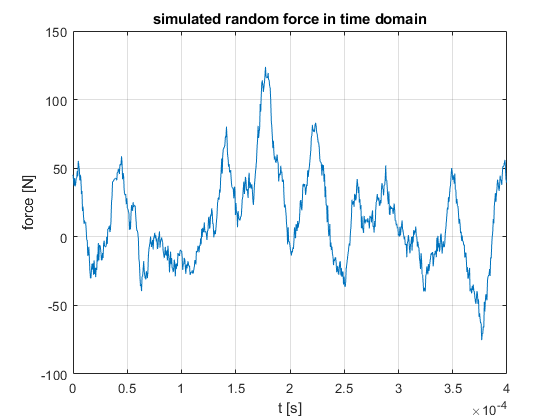
\includegraphics[scale=0.6]{gfx/Force}
		\end{centering}
		\caption{An example of random force to be applied to the tip obtained through the described procedure}
\end{figure}
\subsubsection*{Time lag}
Just before TM release, the two RTs have to exert a force (here considered 0.3N) as low as possible but high enough to control the TM. A time lag between actuation of the two RTs breaks the symmetry of the system, and causes the preload force on one tip to acelerate the TM. In order to evaluate an appropriate value for the lag, a procedure is presented in Bortoluzzi \todo[inline]{bortoluzzi 2}. Trivial computations yield that if push force is constant then it takes $t = 32 \mu s$ to reach the limiting velocity of $5 \nicefrac{\mu m}{s}$. But tip behaviour is unloading spring like (not constant force). Oscillation period is a good evaluation of the time scale of an unloading spring.
\begin{equation*}
T = \frac{2\pi}{\sqrt{\nicefrac{k}{M}}} = 2.2 ms
\end{equation*}
which is far larger than time with constant force. So time lag is modeled with a uniform PDF $30 \mu s$ wide. The time lag is applied to left tip actuation while right tip is always actuated at time $t_0=0$, so the push force is from left to right. This is done for two reasons:
\begin{enumerate}
\item{A time lag on two sides would lead to a symmetric PDF. Computing a one sided one requires half the experiments to perform in the Monte Carlo to obtain the same accuracy}
\item{The time lag statistic properties are simplier, which is convenient for results sensitivity analysis}
\end{enumerate}
\subsubsection*{Integrator choice}
Two criterions have been followed to choose the integration routine.
\begin{enumerate}
\item{The simulation is performed to obtain residual velocity, which is expected to be no larger than $5 \nicefrac{\mu m}{s}$. The result will be than distributed into 50 bins, expeted to be $0.1 \nicefrac{\mu m}{s}$ wide, to compute PDF histogram. Then precision on results must be guaranteed on two decimals only. Therfore the adoption of an integrator of order higher than 3 is useless.} 
\item{Stiffness of RT system is quatified with parameter $S=\nicefrac{\lambda_{max}}{\lambda_{min}}=161$ where $\lambda$ are eigenvalues of the matrix of RT system as it is defined in Sec. 2.1. It is relevant that this value holds for nominal system, while for the real one a small variation occurs. Anyway the system is suspected to be moderately stiff.} 
\end{enumerate}
\todo[inline]{inserire figura autovalori}
The following solvers are considered as good candidates:
\begin{itemize}
\item{\textbf{ode23}: Implements the \textit{Bogacki-Shampine} method, a veriable step explicit RKF order 2 solver with step size control of order 3. The number of function evaluations for each step is 4. It is recommended for non-stiff system when crude tolerances are admissible}
\item{\textbf{ode23s}: A single step solver based on \textit{implicit RK}. Although it requires less time steps than any explicit routine, it may be computationally expensive since number of function evaluation depends on an internal Newton-Rapson subroutine (also needs to compute the jacobian) to solve the implicit equation. Shall be used if the problem is stiff}
\item{\textbf{ode23t}: An implementation of the trapezoidal rule through an interpolant. The method is implicit and an internal simplified Newton subroutine solves the implicit equation, so again the number function evaluations per step is not fixed. It is recommanded for moderately stiff problems}
\item{\textbf{ode23tb}: Similar to the previous one. Applies a \textit{trapezoidal rule} formula for first stage and a \textit{backward interpolation} formula for second stage.}
\end{itemize}
A small Monte Carlo simulation of 50 experiments have been done to test efficiency of integration schemes for solution of this specific problem. Table 4 shows results of this procedure.\\
\begin{table}[h]
\renewcommand{\arraystretch}{1.3}
\begin{tabular}{l||c|c}
\textbf{Integrator} &Number of time steps & CPU time [s]\\ \hline
\textbf{ode23} & 501 & 0.0538\\
\textbf{ode23s} & 88 & 0.0558\\
\textbf{ode23t} & 129 & 0.0275\\
\textbf{ode23tb} & 97 & 0.0202
\end{tabular}
\caption{mean time steps number and mean CPU time for each of the four integration schemes considered}
\end{table}

\section{Results and future work}
\begin{table*}[t]
\setlength{\tabcolsep}{0.75 cm}
\renewcommand{\arraystretch}{1.2}
\begin{tabular}{c| c c c |c c c}
 & \multicolumn{3}{c|}{through parameters covariance} & \multicolumn{3}{c}{through noise filtering}\\
adhesion set used & \textbf{set 1} & \textbf{set 2} & \textbf{set 3} & \textbf{set 1} & \textbf{set 2} & \textbf{set 3}\\ \hline
$V_{res,3\sigma} [\nicefrac{\mu m}{s}]$ & 4.66 & 5.38 & 5.20 & 4.6 & 4.6 & 5.24 \\
$\omega_{res,3\sigma} [\nicefrac{\mu rad}{s}]$ & 2.16 & 2.22 & 2.04 & 2.2 & 2.2 & 2.04
\end{tabular}
\caption{$3\sigma$ linear and angular residual velocities}
\end{table*}
PDF resulting from Monte Carlo simulation are shown in figures \todo[inline]{insert PDF figures numbers}, $3\sigma$ velocities are reported in Table 5.\\
\begin{figure}[H]
		\begin{centering}
			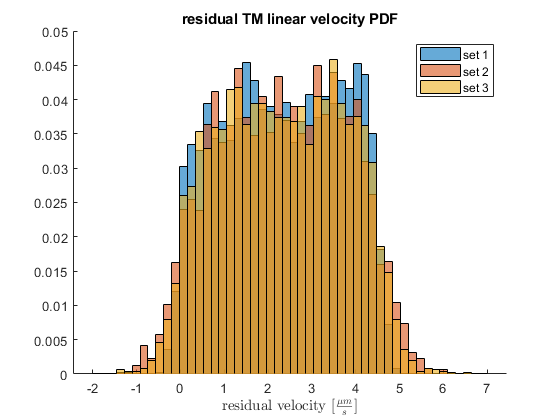
\includegraphics[scale=0.6]{gfx/V_PDF}
		\end{centering}
		\caption{Residual velocity PDF computed through parameters covariance for each of the 3 adhesion sets}
		\label{fig:PDF}
\end{figure}
\begin{figure}[H]
		\begin{centering}
			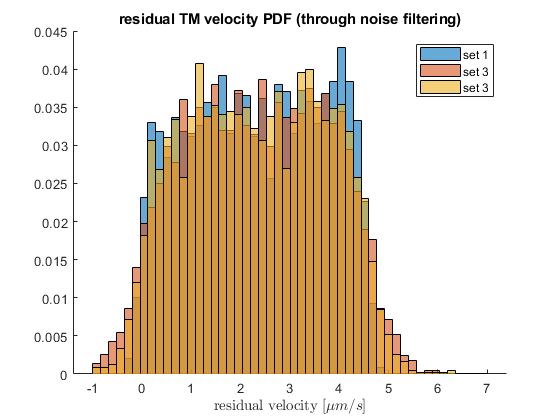
\includegraphics[scale=0.6]{gfx/V_noise_PDF}
		\end{centering}
		\caption{Residual velocity PDF computed through noise filtering for each of the 3 adhesion sets}
\end{figure}
\begin{figure}[H]
		\begin{centering}
			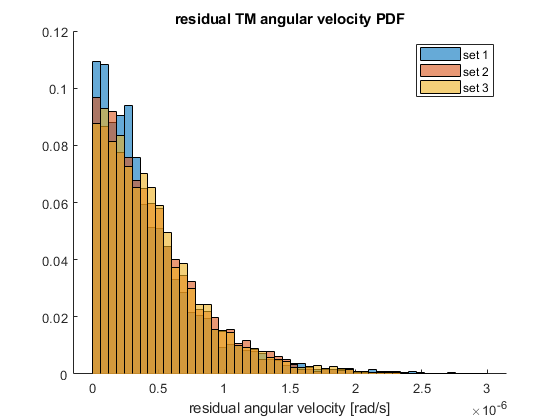
\includegraphics[scale=0.6]{gfx/W_PDF}
		\end{centering}
		\caption{Residual angular velocity PDF computed through parameters covariance for each of the 3 adhesion sets}
\end{figure}
\begin{figure}[H]
		\begin{centering}
			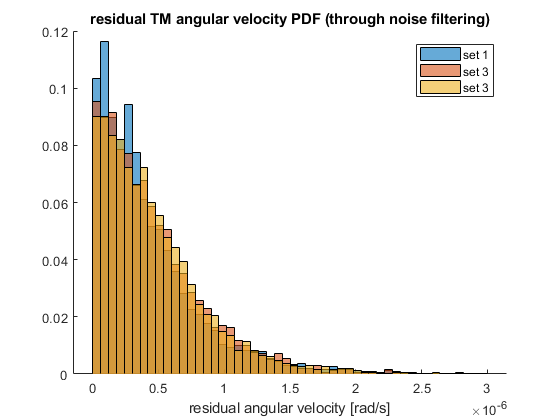
\includegraphics[scale=0.6]{gfx/W_noise_PDF}
		\end{centering}
		\caption{Residual angular velocity PDF computed through noise filtering for each of the 3 adhesion sets}
\end{figure}
Some interesting considerations can be made on the results. It is clear that the two methods used to introduce identification error yield almost equal results, even though they are expected to behave differently, at least for the fact that in the estimation of the covariance matrix an additional standard deviation ($\sigma_{pp} = 0.3\times p$), accounting for \textit{a priori} parameter deviation from nominal ones, have been included. This suggests that parameters deviation from nominal, at least as long as it is bounded under a certain treshold, affects lowly the residual velocities. Effects of adhesion force have been investigated yet (i.e. in Bortoluzzi \todo[inline]{Reference Bortoluzzi 2} and they are low with respect to limiting velocity required. On the contrary effects of preload and time lag are predominant: The PDF in figures  \todo[inline]{insert PDF linear velocity figures numbers} shows a uniform shape. As a matter of fact linear velocity PDF follows the time lag distribution. Fig. \todo[inline]{numero figura sensitivity test} shows how lag time affects residual velocity. Another important result is that as long as the target is to limit velocity to $5 \nicefrac{\mu m}{s}$ effects of prestress are indipendent from parameters and adhesion uncertainties, which is an expected result from considerations done in Sec. 3.2 (\textit{Time lag} subsection). These consideration lead to the result that future design aimed to limit the residual velocity after release within stated constraints specified in tab. 1 will have to focus on reduction of the time lag between RT actuations and of the prerelease load, since this two are by far the most effective parameters on residual quantities.
\begin{figure}[H]
	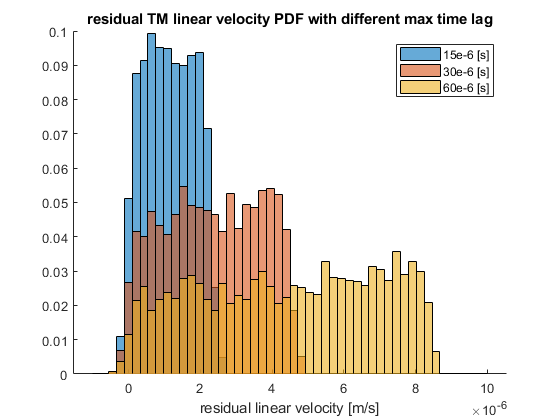
\includegraphics[scale=0.6]{gfx/sens_test}
	\caption{Behaviour of residual velocity PDF generated by different time lags: doubling time lag PDF width doubles the residual velocity one}
\end{figure}

citazione \cite{latexcompanion}
\begin{thebibliography}{9}
\bibitem{latexcompanion} 
Michel Goossens, Frank Mittelbach, and Alexander Samarin. 
\textit{The \LaTeX\ Companion}. 
Addison-Wesley, Reading, Massachusetts, 1993.
 
\bibitem{einstein} 
Albert Einstein. 
\textit{Zur Elektrodynamik bewegter K{\"o}rper}. (German) 
[\textit{On the electrodynamics of moving bodies}]. 

\bibitem{knuthwebsite} 
Knuth: Computers and Typesetting,
\\\texttt{http://www-cs-faculty.stanford.edu/\~{}uno/abcde.html}
\end{thebibliography}
\end{document}